% this document has the propensity to become outdated as the code base
% and results are updated over time. the pdf file should represent the most
% stable implementation of this document.
%
% this is the basic ``template'' for all reports for meetings with ken and to
% send to collaborators.
\documentclass{article}\usepackage{graphicx, color}
%% maxwidth is the original width if it is less than linewidth
%% otherwise use linewidth (to make sure the graphics do not exceed the margin)
\makeatletter
\def\maxwidth{ %
  \ifdim\Gin@nat@width>\linewidth
    \linewidth
  \else
    \Gin@nat@width
  \fi
}
\makeatother

\definecolor{fgcolor}{rgb}{0.2, 0.2, 0.2}
\newcommand{\hlnumber}[1]{\textcolor[rgb]{0,0,0}{#1}}%
\newcommand{\hlfunctioncall}[1]{\textcolor[rgb]{0.501960784313725,0,0.329411764705882}{\textbf{#1}}}%
\newcommand{\hlstring}[1]{\textcolor[rgb]{0.6,0.6,1}{#1}}%
\newcommand{\hlkeyword}[1]{\textcolor[rgb]{0,0,0}{\textbf{#1}}}%
\newcommand{\hlargument}[1]{\textcolor[rgb]{0.690196078431373,0.250980392156863,0.0196078431372549}{#1}}%
\newcommand{\hlcomment}[1]{\textcolor[rgb]{0.180392156862745,0.6,0.341176470588235}{#1}}%
\newcommand{\hlroxygencomment}[1]{\textcolor[rgb]{0.43921568627451,0.47843137254902,0.701960784313725}{#1}}%
\newcommand{\hlformalargs}[1]{\textcolor[rgb]{0.690196078431373,0.250980392156863,0.0196078431372549}{#1}}%
\newcommand{\hleqformalargs}[1]{\textcolor[rgb]{0.690196078431373,0.250980392156863,0.0196078431372549}{#1}}%
\newcommand{\hlassignement}[1]{\textcolor[rgb]{0,0,0}{\textbf{#1}}}%
\newcommand{\hlpackage}[1]{\textcolor[rgb]{0.588235294117647,0.709803921568627,0.145098039215686}{#1}}%
\newcommand{\hlslot}[1]{\textit{#1}}%
\newcommand{\hlsymbol}[1]{\textcolor[rgb]{0,0,0}{#1}}%
\newcommand{\hlprompt}[1]{\textcolor[rgb]{0.2,0.2,0.2}{#1}}%

\usepackage{framed}
\makeatletter
\newenvironment{kframe}{%
 \def\at@end@of@kframe{}%
 \ifinner\ifhmode%
  \def\at@end@of@kframe{\end{minipage}}%
  \begin{minipage}{\columnwidth}%
 \fi\fi%
 \def\FrameCommand##1{\hskip\@totalleftmargin \hskip-\fboxsep
 \colorbox{shadecolor}{##1}\hskip-\fboxsep
     % There is no \\@totalrightmargin, so:
     \hskip-\linewidth \hskip-\@totalleftmargin \hskip\columnwidth}%
 \MakeFramed {\advance\hsize-\width
   \@totalleftmargin\z@ \linewidth\hsize
   \@setminipage}}%
 {\par\unskip\endMakeFramed%
 \at@end@of@kframe}
\makeatother

\definecolor{shadecolor}{rgb}{.97, .97, .97}
\definecolor{messagecolor}{rgb}{0, 0, 0}
\definecolor{warningcolor}{rgb}{1, 0, 1}
\definecolor{errorcolor}{rgb}{1, 0, 0}
\newenvironment{knitrout}{}{} % an empty environment to be redefined in TeX

\usepackage{alltt}
\usepackage{amsmath, amsthm}
\usepackage{graphicx, microtype, parskip}
\usepackage{rotating, longtable, caption, subcaption}
\usepackage[sort&compress]{natbib}

\frenchspacing




\begin{knitrout}
\definecolor{shadecolor}{rgb}{1, 1, 1}\color{fgcolor}\begin{kframe}


{\ttfamily\noindent\bfseries\color{errorcolor}{\#\# Error: cannot open the connection}}\end{kframe}
\end{knitrout}


\begin{knitrout}
\definecolor{shadecolor}{rgb}{1, 1, 1}\color{fgcolor}\begin{kframe}


{\ttfamily\noindent\bfseries\color{errorcolor}{\#\# Error: object 'turtle.train' not found}}

{\ttfamily\noindent\bfseries\color{errorcolor}{\#\# Error: object 'turtle.test' not found}}

{\ttfamily\noindent\bfseries\color{errorcolor}{\#\# Error: object 'turtle.train' not found}}\end{kframe}
\end{knitrout}


\title{How cryptic is cryptic diversity? Machine learning approaches to fine scale variation in the morphology of \textit{Emys marmorata}.}
\IfFileExists{upquote.sty}{\usepackage{upquote}}{}

\begin{document}
\maketitle


\section{Methods}
No-free lunch theorem. Try lots of things because we don't understand everything.

\subsection{Unsupervised}
Underlying structure in data?

\subsubsection{Gap-based clustering}
Comparison of gap statistic results for partitioning around medoids (PAM) divisive clustering. Confidence intervals are determined via bootstrap. The higher the gap statistic, the better the clustering result. Standard errors of the gap statistic were estimated from 100 resamples.


\subsubsection{Evidence Accumulation Clustering}
Choosing an optimal number of partitions is hard, which is why gap-based cluster selection was used above. An alternative method is to look at the co-occurrence frequency, that is how frequently any two samples occur in the same partition. Repeating this process over and over again creates the frequency, or ``vote'' for how the data set should be partitioned and  which specimens should be in the same cluster.

EAC was originally devised using \textit{k}-means clustering, but I've extended it to use PAM clustering instead. The hope is to determine underlying structure in the data given a wide enough partition range and a high enough number of iterations. Dissimilarity based EAC was performed using a range of 1 though 200 possible partitions and based on 10,000 iterations.

\subsection{Supervised}
How well does data conform to predetermined structure?

\begin{itemize}
  \item multinomial logistic regression (Fig. \ref{fig:multi-map})
  \item feed-forward neural networks (Fig. \ref{fig:nnet-map})
  \item random forests (Fig. \ref{fig:rf-map})
\end{itemize}


\section{Preliminary results}
\subsection{Unsupervised}
Comparison of gap statistic over a very wide range of plausible partitions indicates that as the number of partitions increase, there is a marginal increasing gap statistic until approximately 

{\ttfamily\noindent\bfseries\color{errorcolor}{\\Error in eval(expr, envir, enclos) : object 'tmorph.km' not found}} after which there is a marginal decrease in gap statistic (Fig. \ref{fig:gap}). It is notable that the standard errors around the gap statistic values are very large, and the marginal increases in gap statistic with an increased number of partitions may not be important. Additionally, all gap statistic values are within 

{\ttfamily\noindent\bfseries\color{errorcolor}{\\Error in eval(expr, envir, enclos) : object 'tmorph.gap' not found}} of each other meaning that there is little over all consensus for how many clusters are present when comparing gap statistics.

\begin{knitrout}
\definecolor{shadecolor}{rgb}{1, 1, 1}\color{fgcolor}\begin{kframe}


{\ttfamily\noindent\bfseries\color{errorcolor}{\#\# Error: object 'tmorph.gap' not found}}

{\ttfamily\noindent\bfseries\color{errorcolor}{\#\# Error: object 'gg.gap' not found}}\end{kframe}
\end{knitrout}

\begin{figure}[ht]
  \centering
  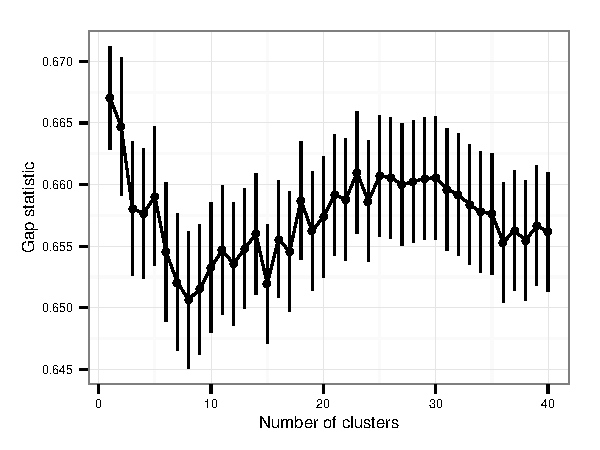
\includegraphics[width = \textwidth, keepaspectratio = true]{figure/gap}
  \caption{Gap statistic values for multiple PAM-based clustering configurations of the Riemmanian shape distances of the \textit{Emys marmorata} plastra. Higher values indicate greater clustering. Standard errors are estimated from 100 bootstrap resamples.}
  \label{fig:gap}
\end{figure}

\begin{knitrout}
\definecolor{shadecolor}{rgb}{1, 1, 1}\color{fgcolor}\begin{kframe}


{\ttfamily\noindent\bfseries\color{errorcolor}{\#\# Error: object 'tadult.gap' not found}}

{\ttfamily\noindent\bfseries\color{errorcolor}{\#\# Error: object 'ad.gap' not found}}\end{kframe}
\end{knitrout}



Dissimilarity based EAC estimated approximately 

{\ttfamily\noindent\bfseries\color{errorcolor}{\\Error in eval(expr, envir, enclos) : object 'tmorph.dac' not found}} optimal partitions (Table \ref{tab:dac}) though this may be only a marginal difference. I need to increase the number of resamples from 100 to 500 because that is when approximate stability is estimated to occur. 

\begin{kframe}


{\ttfamily\noindent\bfseries\color{errorcolor}{\#\# Error: object 'tmorph.dac' not found}}

{\ttfamily\noindent\bfseries\color{errorcolor}{\#\# Error: object 'dac.tab' not found}}

{\ttfamily\noindent\bfseries\color{errorcolor}{\#\# Error: object 'dac.tab' not found}}

{\ttfamily\noindent\bfseries\color{errorcolor}{\#\# Error: object 'dac.tab' not found}}\end{kframe}


Here is the PCA plot of the turtle pastra (Fig. \ref{fig:gm}). Also included is the mean shape and the dispersion around the landmarks. I haven't put nay classification labels on the points because an optimal partition scheme has not been selected.

\begin{knitrout}
\definecolor{shadecolor}{rgb}{1, 1, 1}\color{fgcolor}\begin{kframe}


{\ttfamily\noindent\bfseries\color{errorcolor}{\#\# Error: object 'turtle.info' not found}}

{\ttfamily\noindent\bfseries\color{errorcolor}{\#\# Error: object 'turtle.land.info' not found}}

{\ttfamily\noindent\bfseries\color{errorcolor}{\#\# Error: object 'fits' not found}}

{\ttfamily\noindent\bfseries\color{errorcolor}{\#\# Error: object 'gg.morph' not found}}

{\ttfamily\noindent\bfseries\color{errorcolor}{\#\# Error: object 'gg.morph' not found}}\end{kframe}
\end{knitrout}


\begin{figure}[ht]
  \centering
  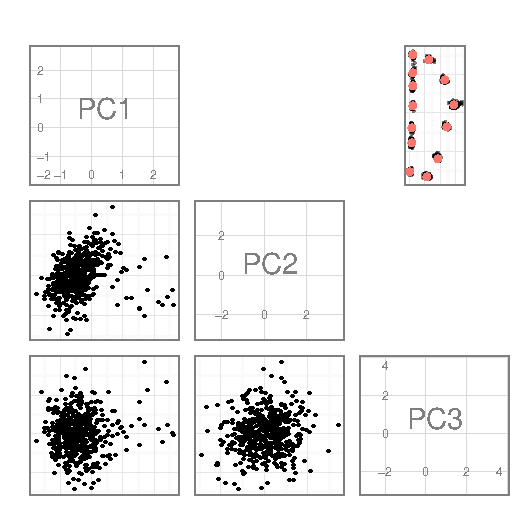
\includegraphics[width = \textwidth]{figure/gm}
  \caption{Visualization of PCA of \textit{E. marmorata}. The lower triangle is the pairwise comparison of the first three principal components. The upper left corner is the comparison of landmark dispersion for all specimens compared to the mean shape in red.}
  \label{fig:gm}
\end{figure}


\subsection{Supervised}

\subsubsection{Model selection}
% multinomial logistic regression AICc tables
%
% nnet recursive feature selection
%
% random forest recursive feature selection

I'm currently holding back on showing all the tables and model selection procedures because there are a lot of them. I'll show the confusion matrices from the multinomial logistic regressions because they are easy (Tables \ref{tab:multi-conf-sh1}, \ref{tab:multi-conf-sh2}, \ref{tab:multi-conf-sh3}, \ref{tab:multi-conf-spinks}). The confusion matrices from the neural network and random forest models are easy to make too, just would increase the overall length of this document by quite a bit.

\begin{kframe}


{\ttfamily\noindent\bfseries\color{errorcolor}{\#\# Error: object 'tm.conf' not found}}

{\ttfamily\noindent\bfseries\color{errorcolor}{\#\# Error: object 'mt' not found}}

{\ttfamily\noindent\bfseries\color{errorcolor}{\#\# Error: object 'mt' not found}}\end{kframe}


But I can show the comparison of the predictive accuracies (Fig. \ref{fig:resamp}).

\begin{knitrout}
\definecolor{shadecolor}{rgb}{1, 1, 1}\color{fgcolor}\begin{kframe}


{\ttfamily\noindent\bfseries\color{errorcolor}{\#\# Error: object 'tmod.re' not found}}

{\ttfamily\noindent\bfseries\color{errorcolor}{\#\# Error: object 'tmod.re.clean' not found}}

{\ttfamily\noindent\bfseries\color{errorcolor}{\#\# Error: object 'tmod.re.gg' not found}}\end{kframe}
\end{knitrout}


\begin{figure}[t]
  \centering
  \begin{subfigure}[b]{0.5\textwidth}
    \centering
    \caption{}
    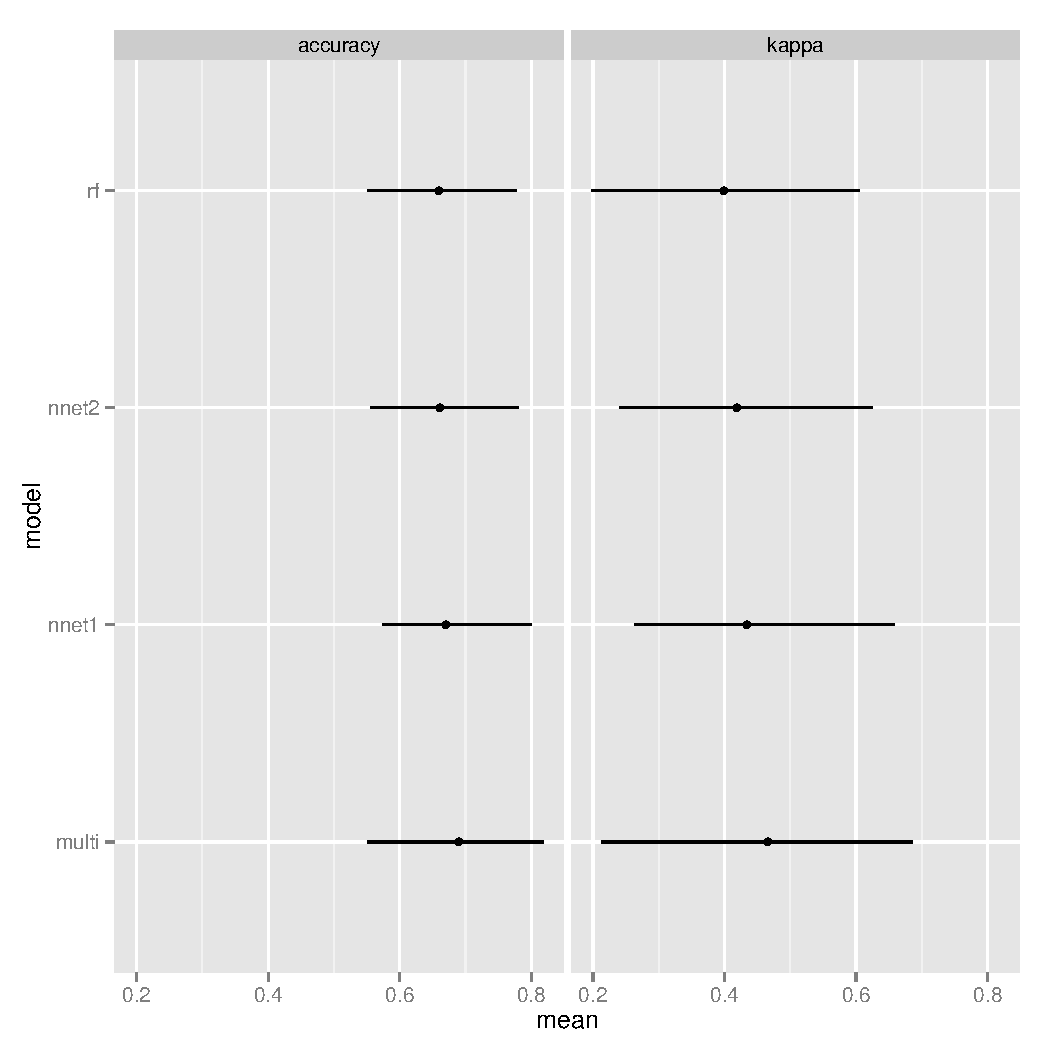
\includegraphics[width = \textwidth]{figure/resamp1}
    \label{fig:resamp1}
  \end{subfigure}%
  \begin{subfigure}[b]{0.5\textwidth}
    \centering
    \caption{}
    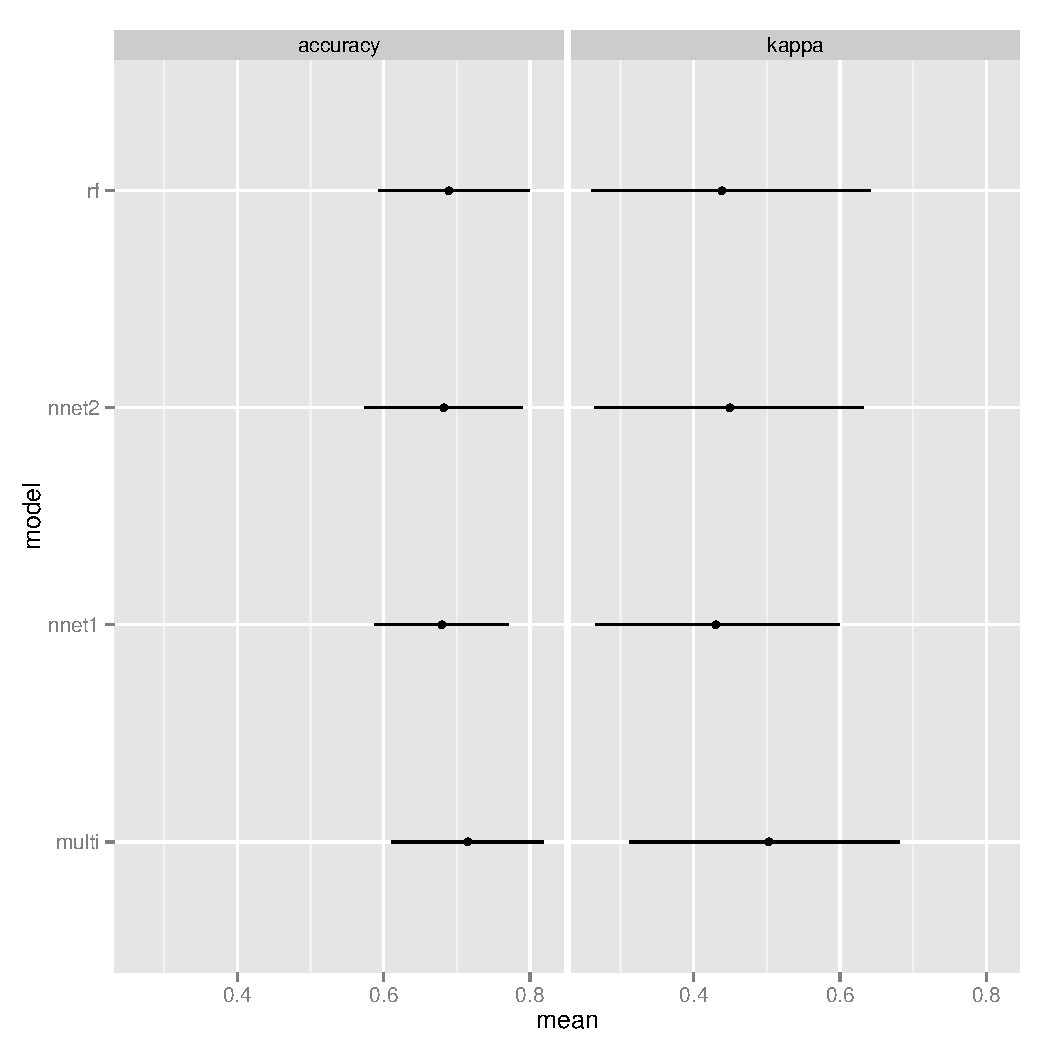
\includegraphics[width = \textwidth]{figure/resamp2}
    \label{fig:resamp2}
  \end{subfigure}\\

  \begin{subfigure}[b]{0.5\textwidth}
    \centering
    \caption{}
    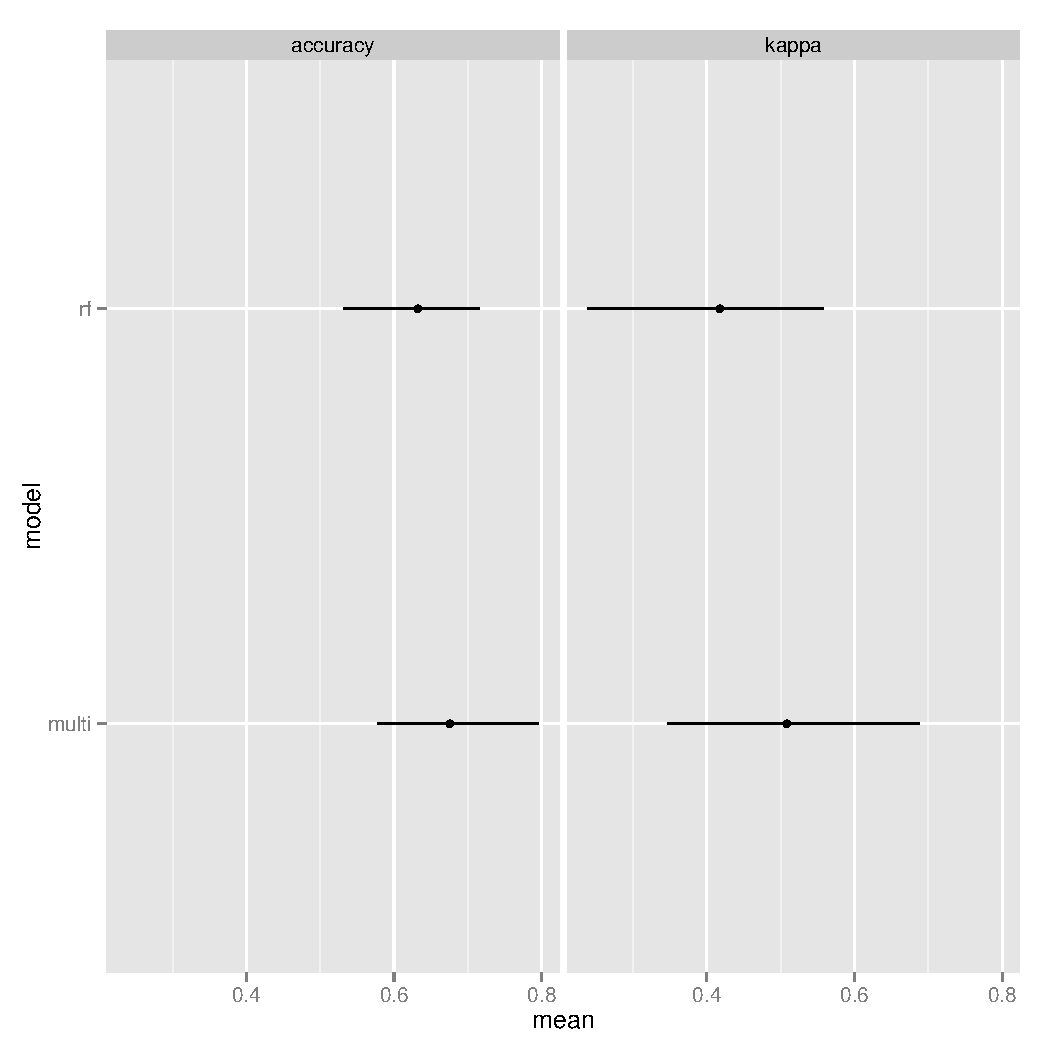
\includegraphics[width = \textwidth]{figure/resamp3}
    \label{fig:resamp3}
  \end{subfigure}%
  \begin{subfigure}[b]{0.5\textwidth}
    \centering
    \caption{}
    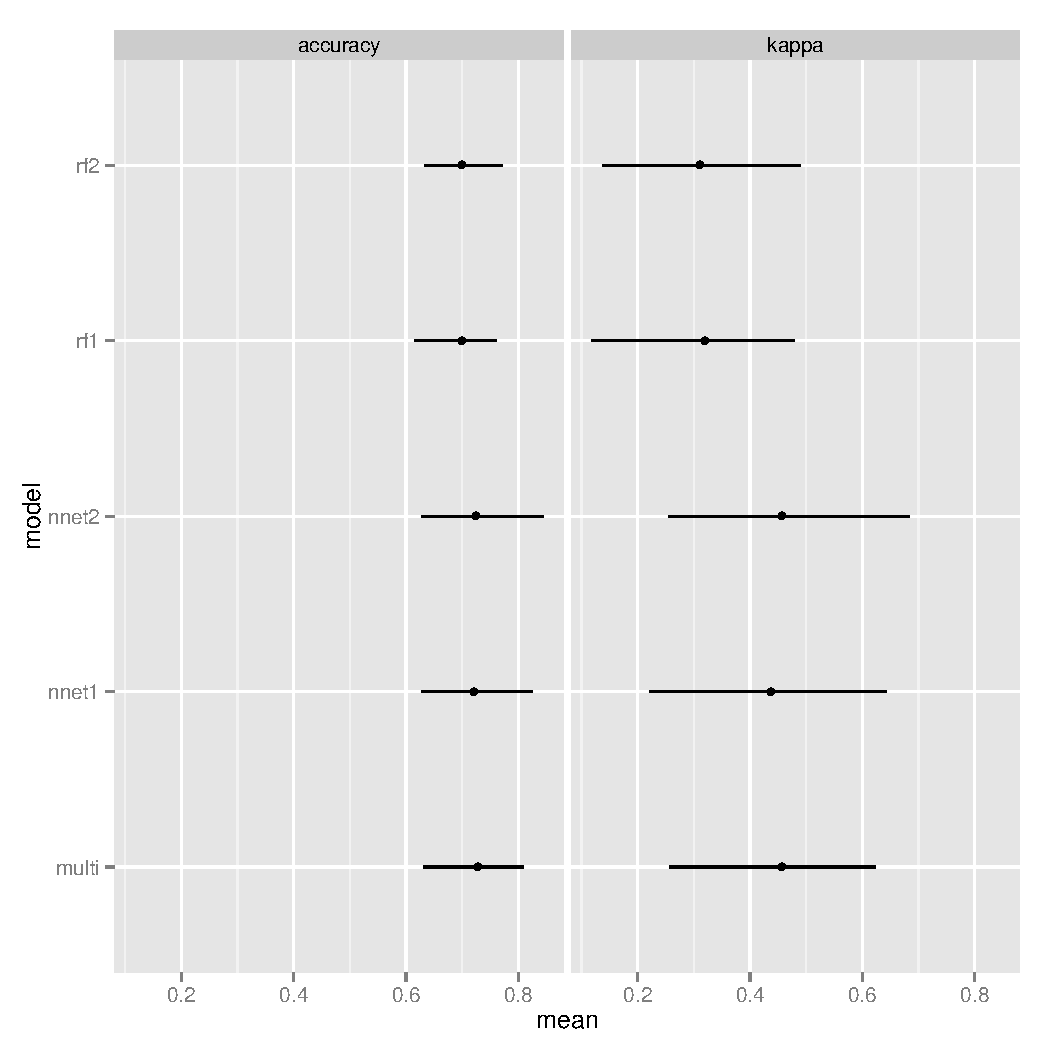
\includegraphics[width = \textwidth]{figure/resamp4}
    \label{fig:resamp4}
  \end{subfigure}
  \caption{Comparison of resampling distributions of training set accuracy and kappa statistics for the selected models of each classification scheme. \ref{fig:resamp1}: sh1 classification scheme. \ref{fig:resamp2}: sh2 classification scheme. \ref{fig:resamp3}: sh3 classification scheme. \ref{fig:resamp4}: spinks classification scheme.}
  \label{fig:resamp}
\end{figure}


In the interest of space/time, I'm only going to display results from one of the selected models from each method for each classification scheme.

\begin{knitrout}
\definecolor{shadecolor}{rgb}{1, 1, 1}\color{fgcolor}\begin{kframe}


{\ttfamily\noindent\bfseries\color{errorcolor}{\#\# Error: object 'turtle.train' not found}}

{\ttfamily\noindent\bfseries\color{errorcolor}{\#\# Error: object 'tm.map' not found}}\end{kframe}
\end{knitrout}


\begin{figure}[t]
  \centering
  \begin{subfigure}[b]{0.5\textwidth}
    \centering
    \caption{}
    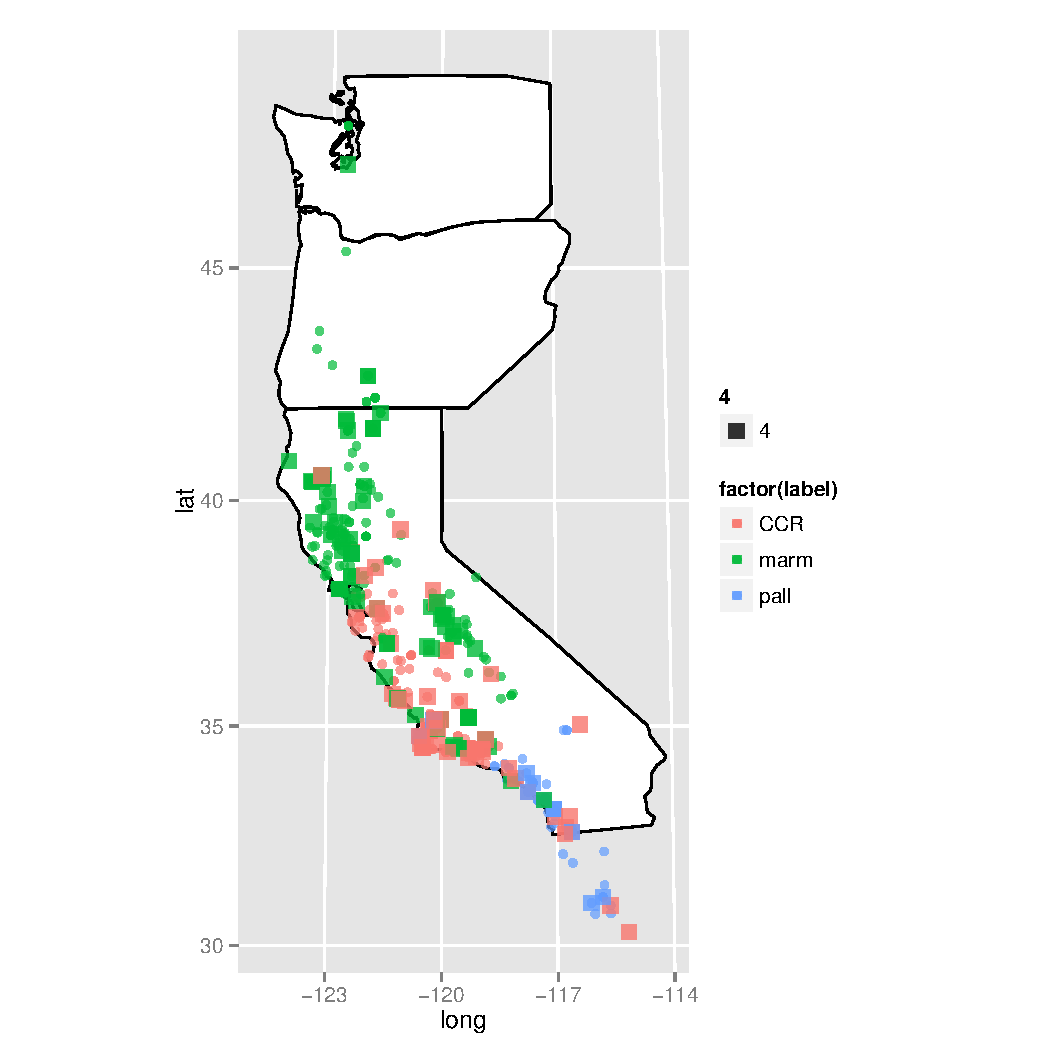
\includegraphics[width = \textwidth]{figure/multi-map1}
    \label{fig:multi-map1}
  \end{subfigure}%
  \begin{subfigure}[b]{0.5\textwidth}
    \centering
    \caption{}
    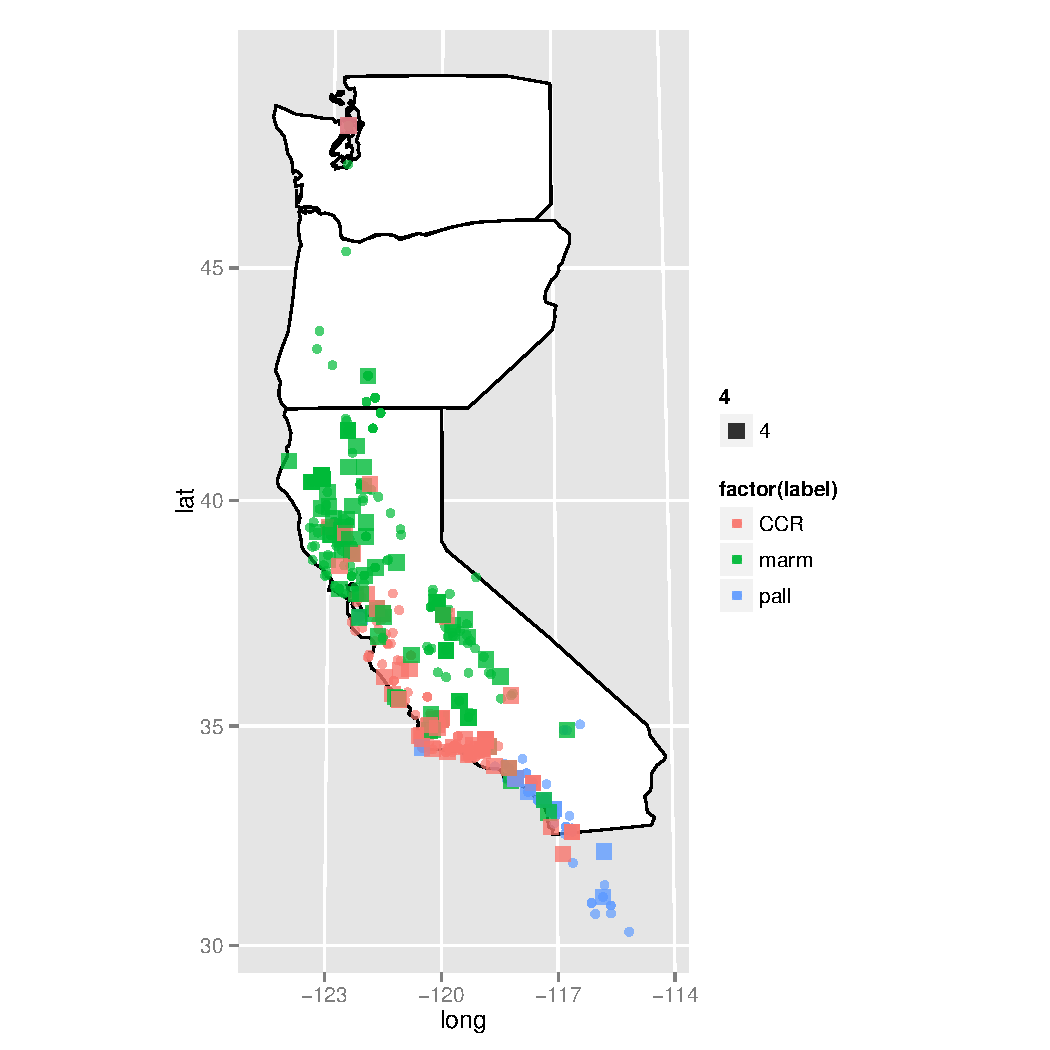
\includegraphics[width = \textwidth]{figure/multi-map2}
    \label{fig:multi-map2}
  \end{subfigure}\\

  \begin{subfigure}[b]{0.5\textwidth}
    \centering
    \caption{}
    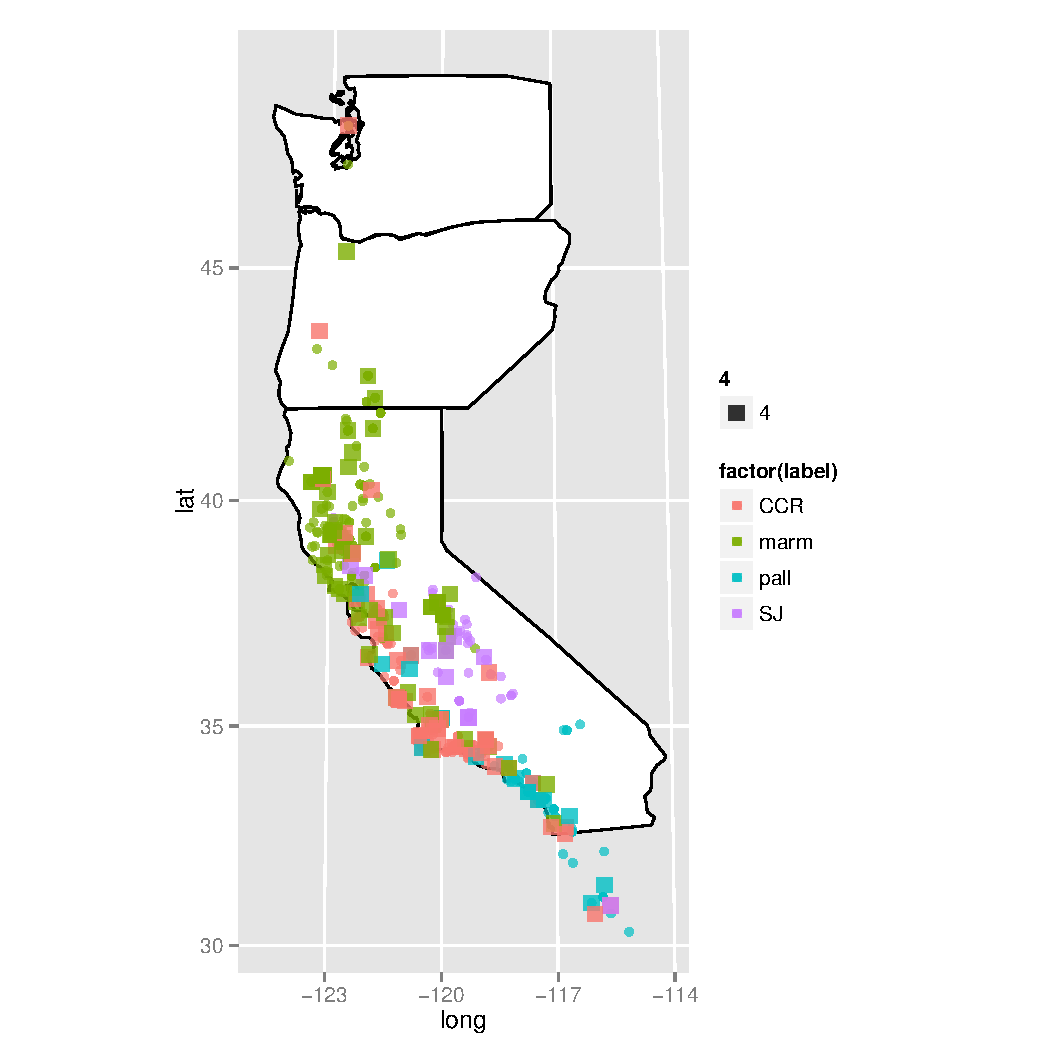
\includegraphics[width = \textwidth]{figure/multi-map3}
    \label{fig:multi-map3}
  \end{subfigure}%
  \begin{subfigure}[b]{0.5\textwidth}
    \centering
    \caption{}
    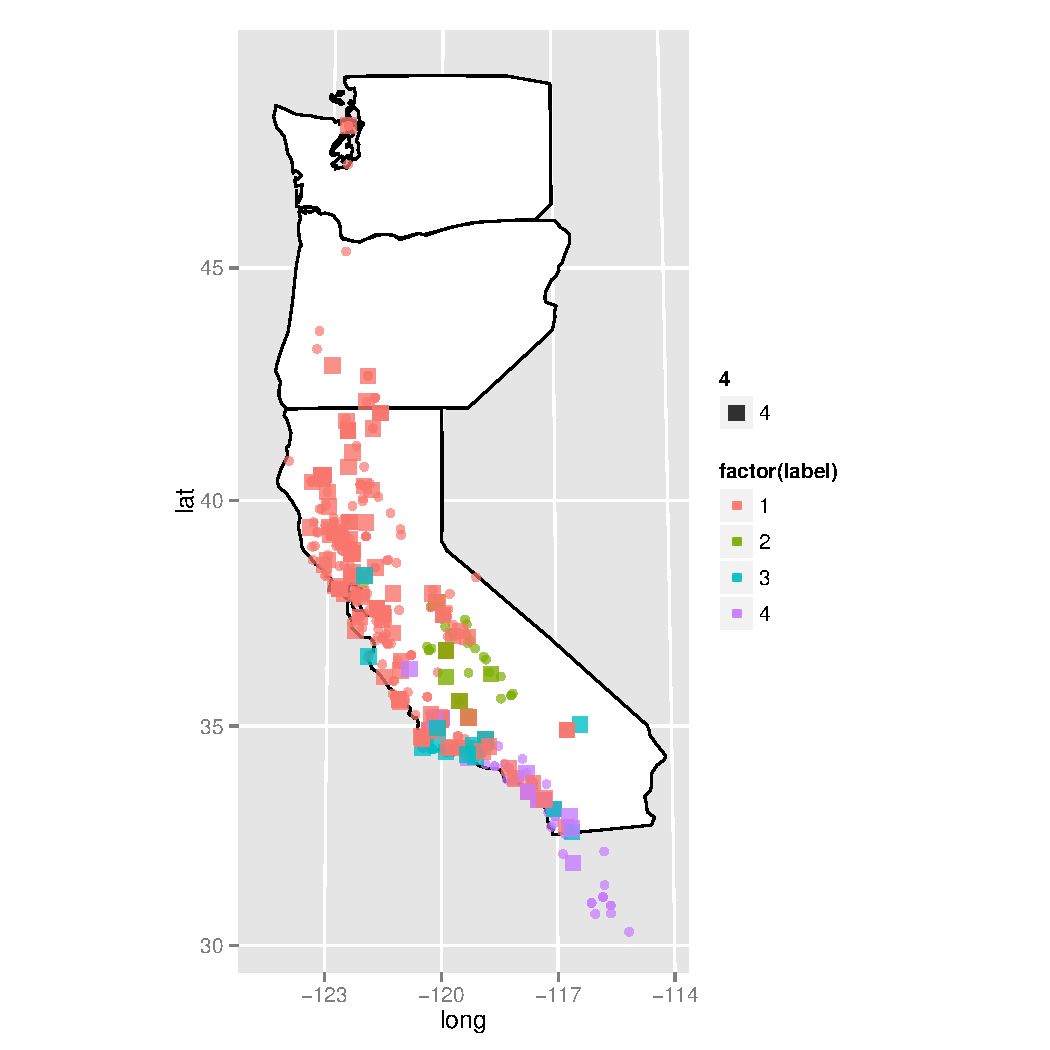
\includegraphics[width = \textwidth]{figure/multi-map4}
    \label{fig:multi-map4}
  \end{subfigure}
  \caption{Geographic position of all turtles sampled. Both training and testing observations are plotted. Training set observations are circles while testing observations are larger squares. Testing set observations are classified based on a multinomial logistic regression model. \ref{fig:multi-map1}: sh1 classification scheme. \ref{fig:multi-map2}: sh2 classification scheme. \ref{fig:multi-map3}: sh3 classification scheme. \ref{fig:multi-map4}: spinks classification scheme.}
  \label{fig:multi-map}
\end{figure}




\begin{figure}[t]
  \centering
  \begin{subfigure}[b]{0.5\textwidth}
    \centering
    \caption{}
    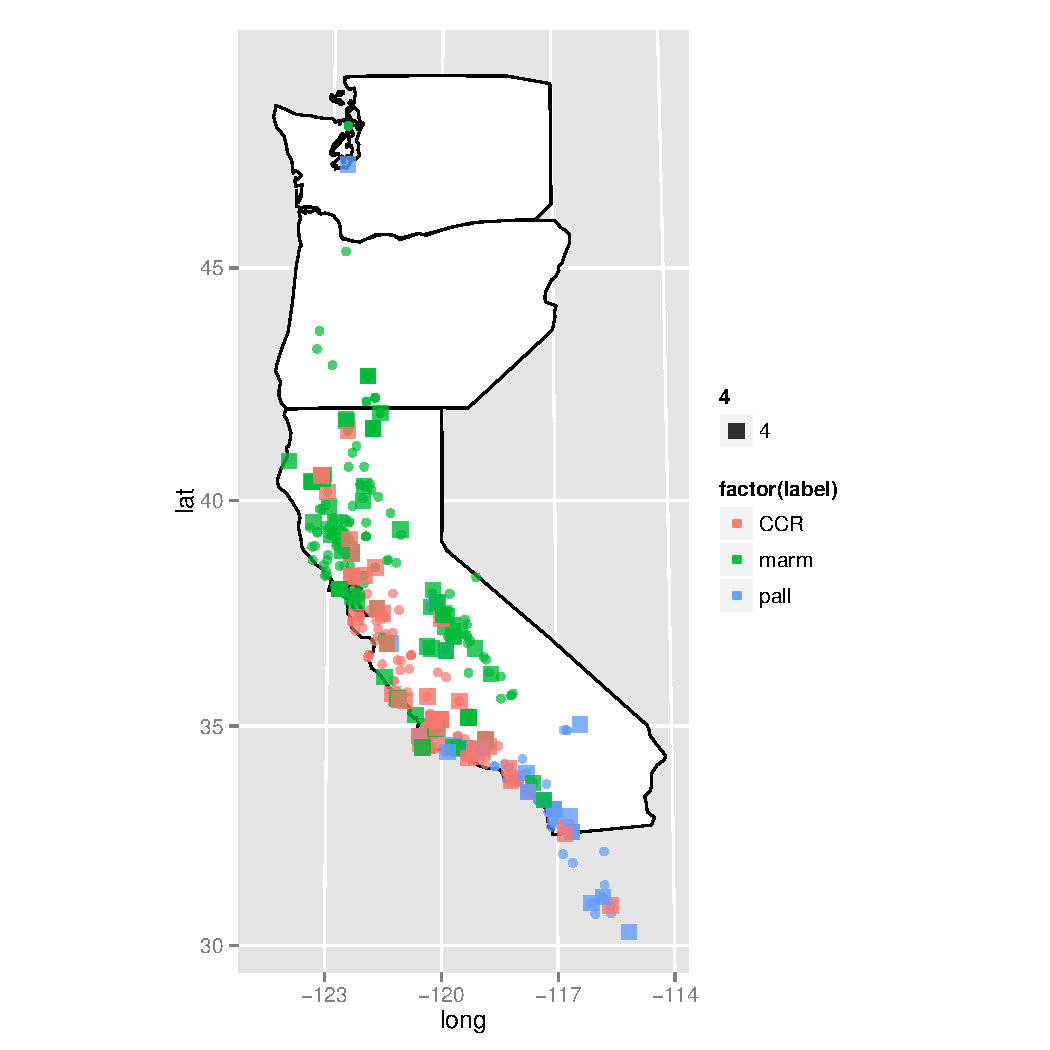
\includegraphics[width = \textwidth]{figure/nnet-map1}
    \label{fig:nnet-map1}
  \end{subfigure}%
  \begin{subfigure}[b]{0.5\textwidth}
    \centering
    \caption{}
    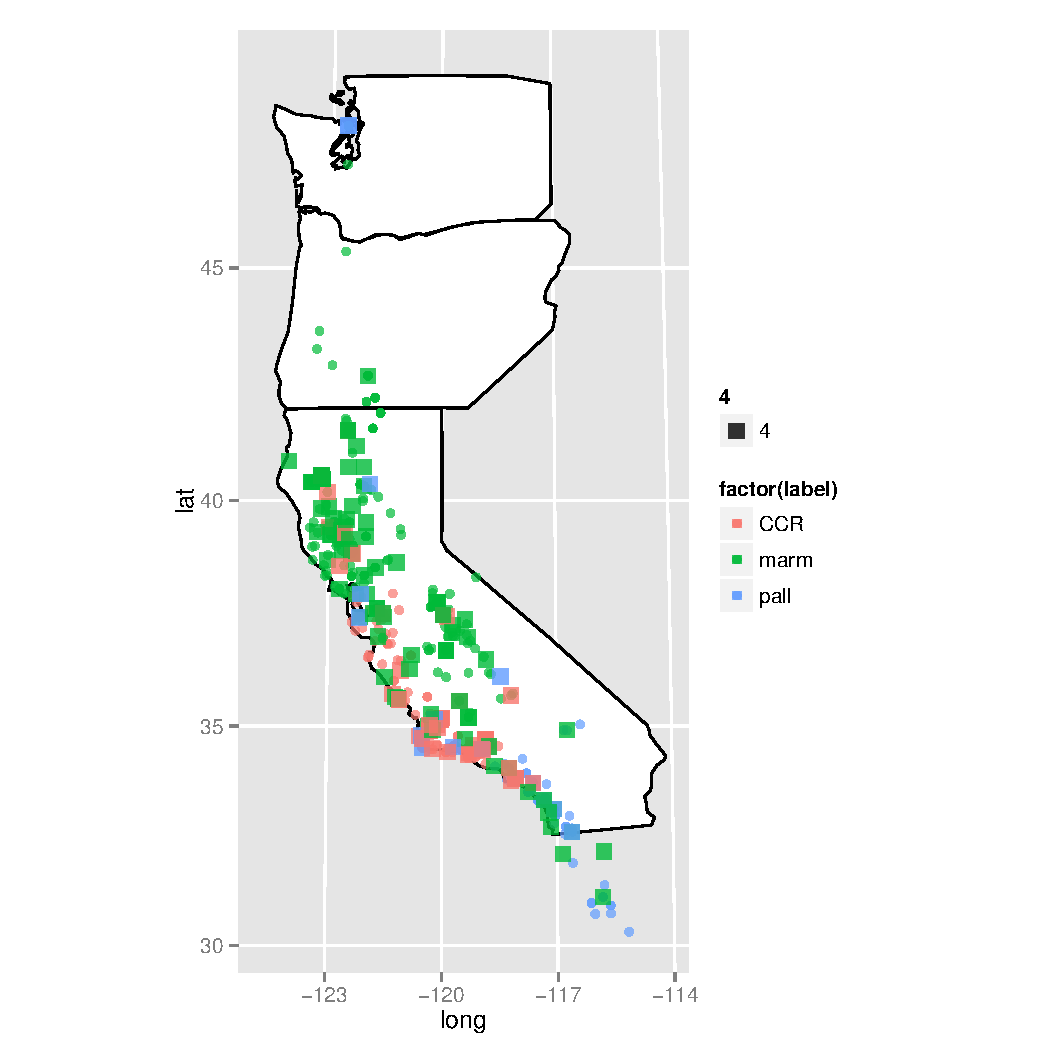
\includegraphics[width = \textwidth]{figure/nnet-map2}
    \label{fig:nnet-map2}
  \end{subfigure}\\

  \begin{subfigure}[b]{0.5\textwidth}
    \centering
    \caption{}
    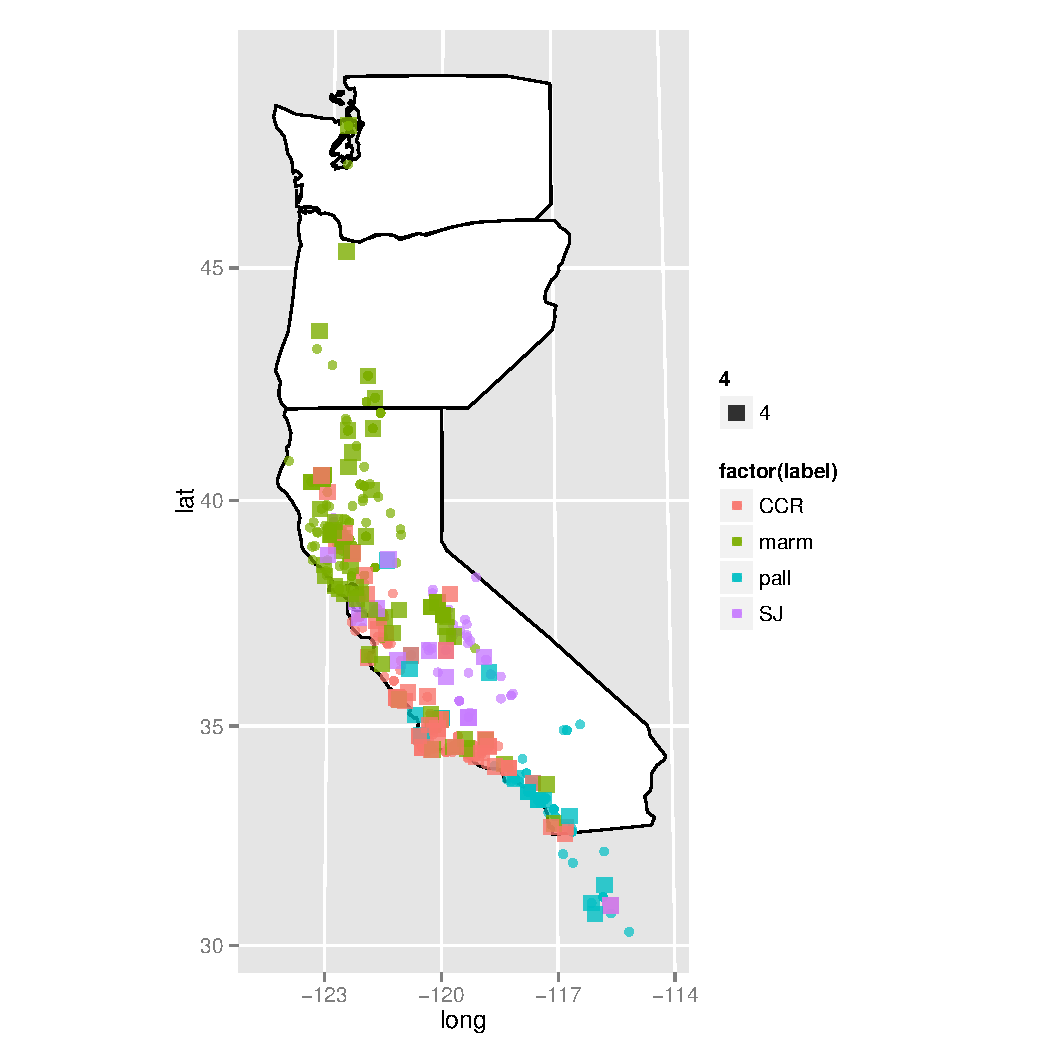
\includegraphics[width = \textwidth]{figure/nnet-map3}
    \label{fig:nnet-map3}
  \end{subfigure}%
  \begin{subfigure}[b]{0.5\textwidth}
    \centering
    \caption{}
    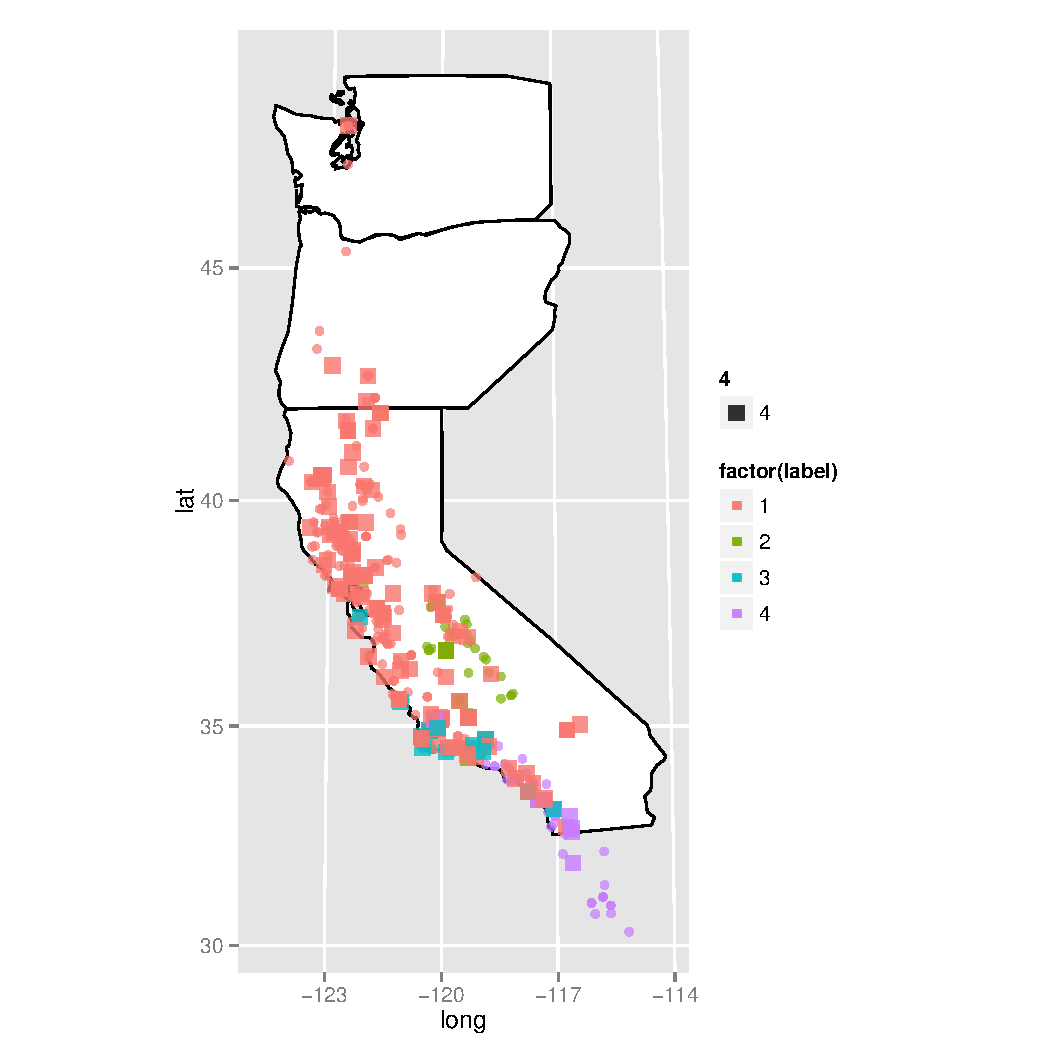
\includegraphics[width = \textwidth]{figure/nnet-map4}
    \label{fig:nnet-map4}
  \end{subfigure}
  \caption{Geographic position of all turtles sampled. Both training and testing observations are plotted. Training set observations are circles while testing observations are larger squares. Testing set observations are classified based on a feed-forward single layer neural network model. \ref{fig:nnet-map1}: sh1 classification scheme. \ref{fig:nnet-map2}: sh2 classification scheme. \ref{fig:nnet-map3}: sh3 classification scheme. \ref{fig:nnet-map4}: spinks classification scheme.}
  \label{fig:nnet-map}
\end{figure}


\begin{knitrout}
\definecolor{shadecolor}{rgb}{1, 1, 1}\color{fgcolor}\begin{kframe}


{\ttfamily\noindent\bfseries\color{errorcolor}{\#\# Error: object 'trf.class' not found}}

{\ttfamily\noindent\bfseries\color{errorcolor}{\#\# Error: object 'turtle.train' not found}}

{\ttfamily\noindent\bfseries\color{errorcolor}{\#\# Error: object 'trf.map' not found}}\end{kframe}
\end{knitrout}


\begin{figure}[t]
  \centering
  \begin{subfigure}[b]{0.5\textwidth}
    \centering
    \caption{}
    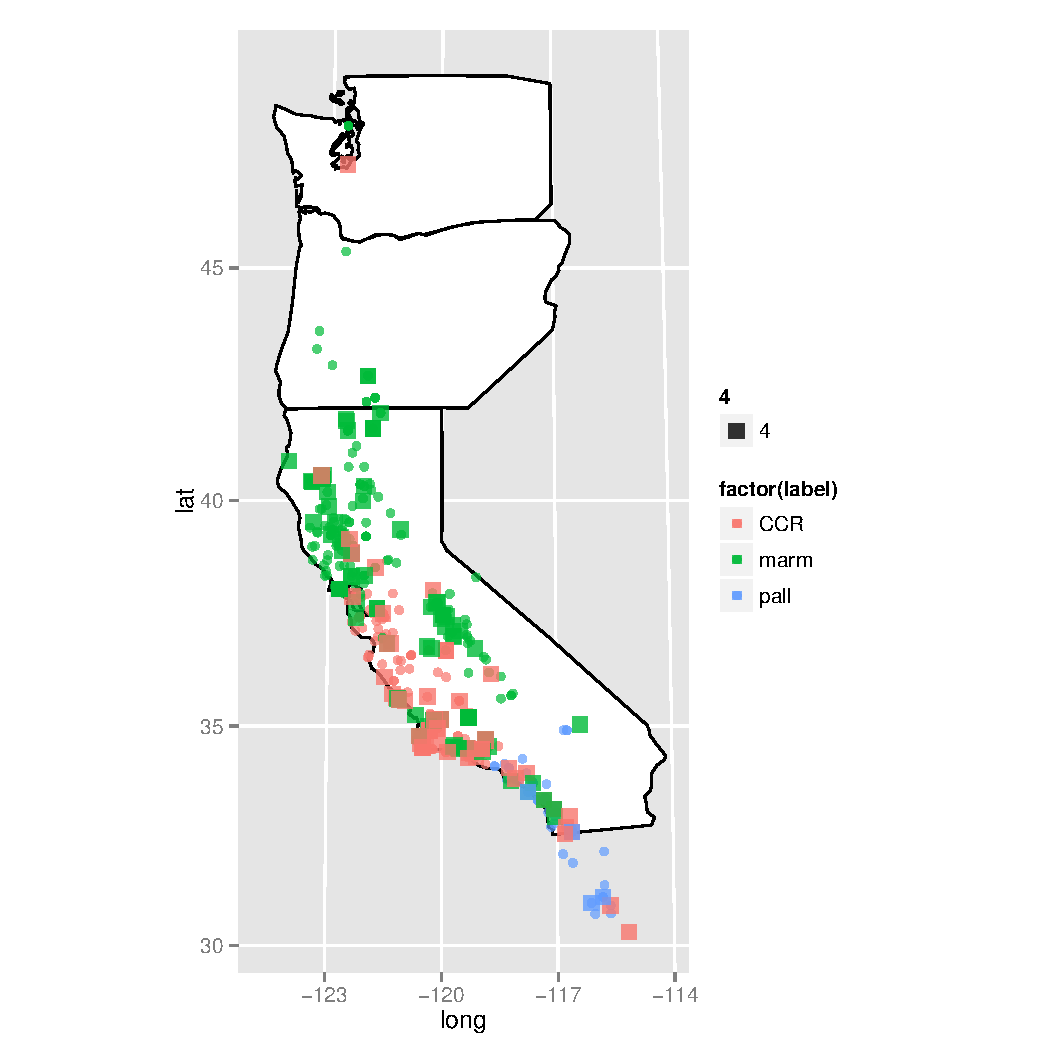
\includegraphics[width = \textwidth]{figure/rf-map1}
    \label{fig:rf-map1}
  \end{subfigure}%
  \begin{subfigure}[b]{0.5\textwidth}
    \centering
    \caption{}
    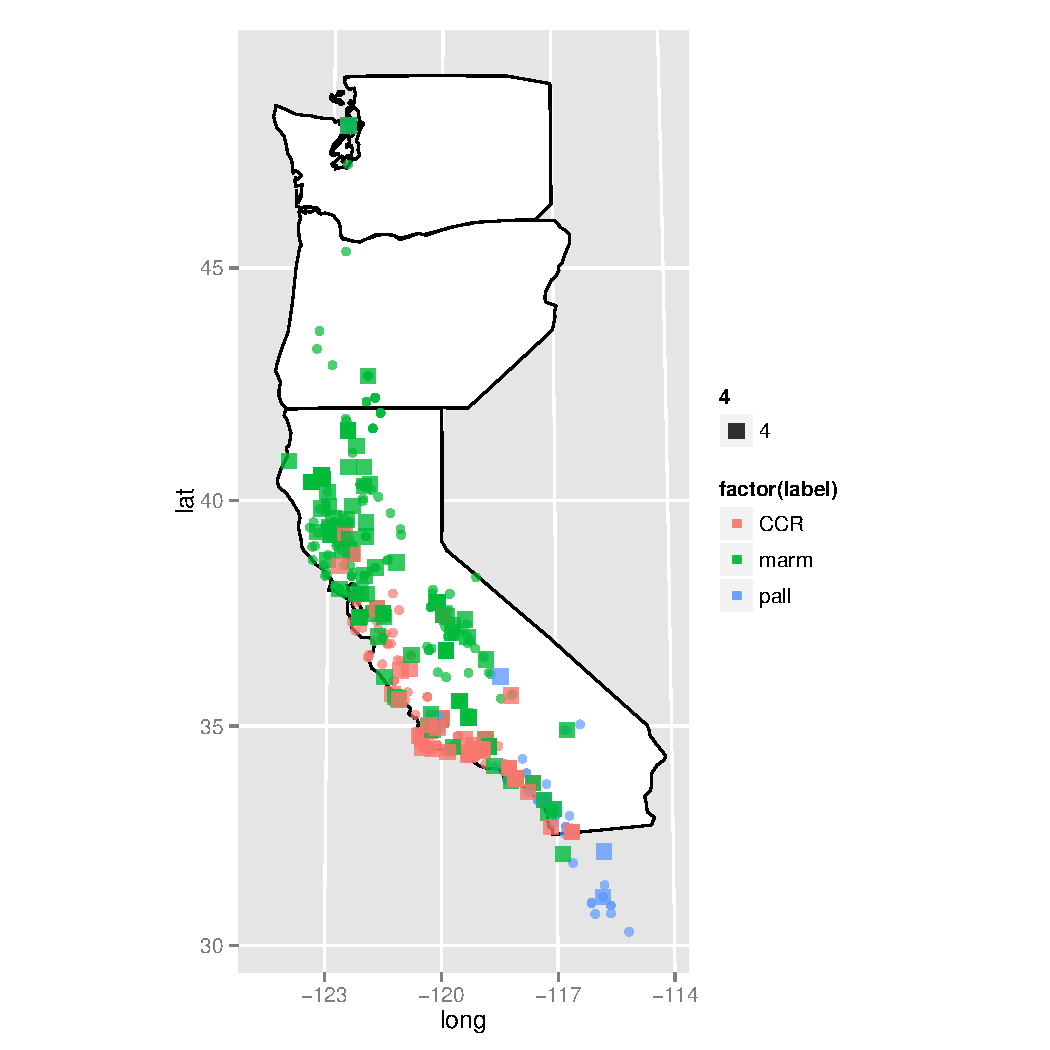
\includegraphics[width = \textwidth]{figure/rf-map2}
    \label{fig:rf-map2}
  \end{subfigure}\\

  \begin{subfigure}[b]{0.5\textwidth}
    \centering
    \caption{}
    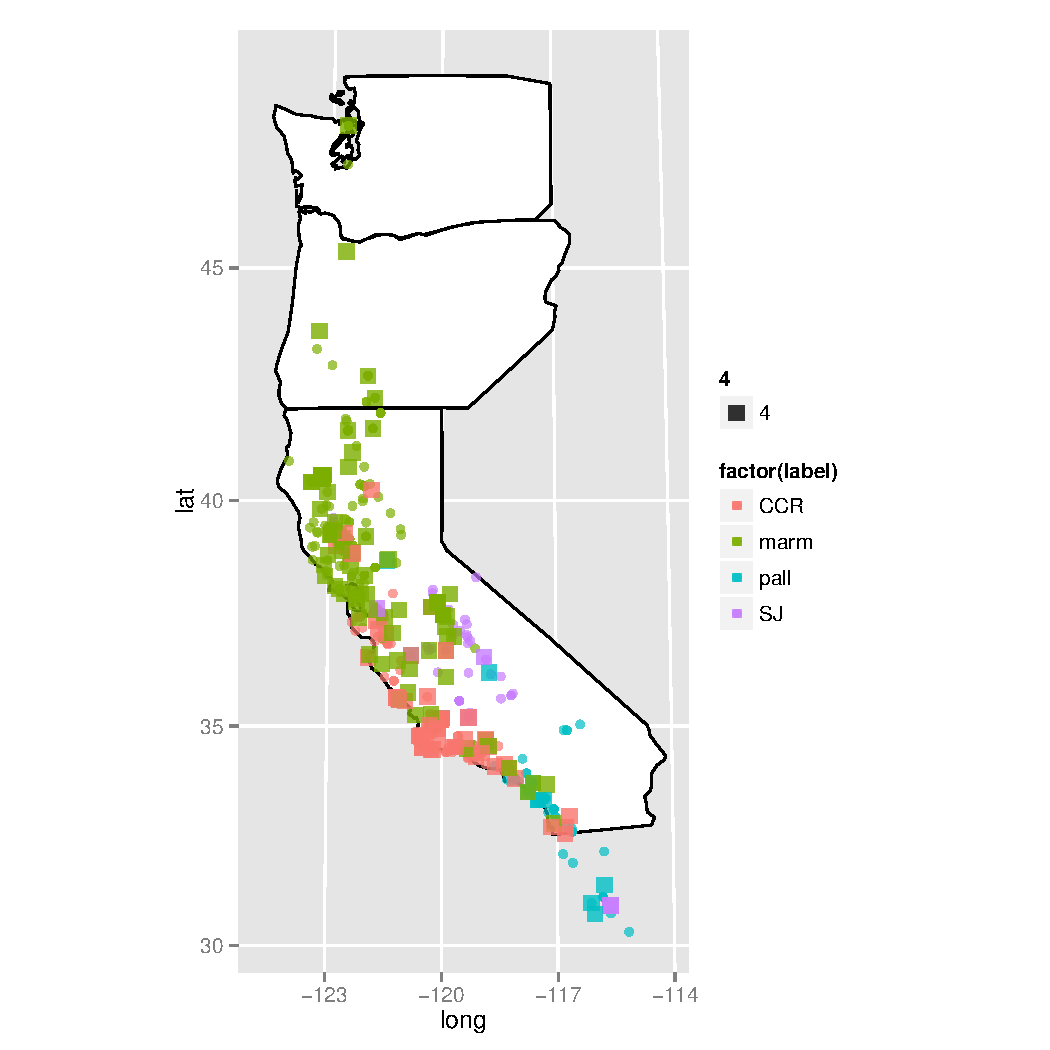
\includegraphics[width = \textwidth]{figure/rf-map3}
    \label{fig:rf-map3}
  \end{subfigure}%
  \begin{subfigure}[b]{0.5\textwidth}
    \centering
    \caption{}
    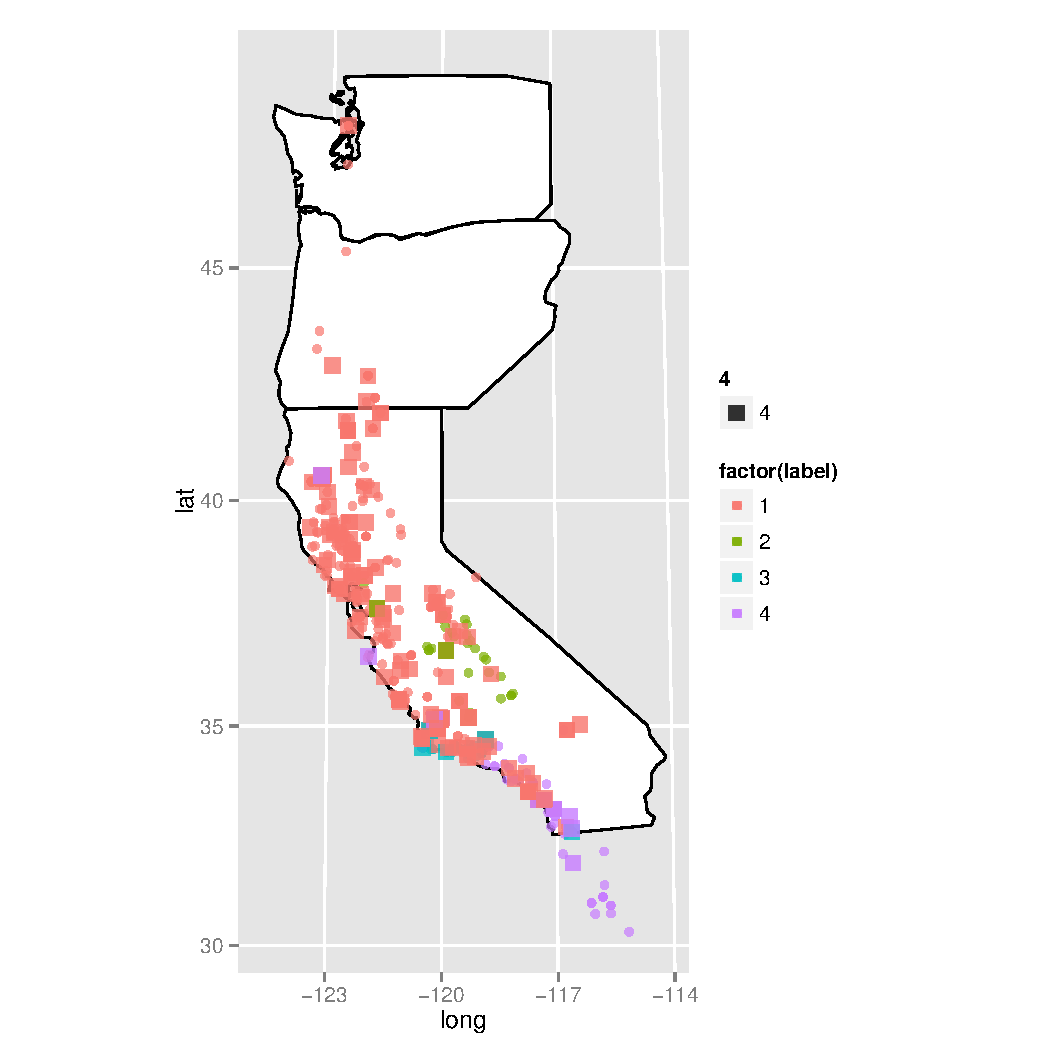
\includegraphics[width = \textwidth]{figure/rf-map4}
    \label{fig:rf-map4}
  \end{subfigure}
  \caption{Geographic position of all turtles sampled. Both training and testing observations are plotted. Training set observations are circles while testing observations are larger squares. Testing set observations are classified based on a random forest model. \ref{fig:rf-map1}: sh1 classification scheme. \ref{fig:rf-map2}: sh2 classification scheme. \ref{fig:rf-map3}: sh3 classification scheme. \ref{fig:rf-map4}: spinks classification scheme.}
  \label{fig:rf-map}
\end{figure}


\section{Future}
\begin{enumerate}
  \item remove juveniles
  \item look into multinomial logistic mixed-effects models
  \item other unsupervised methods, though that might have to wait for a follow up paper
    \begin{itemize}
      \item bayesian nonparametrics for categorical data. Probably the best option and most interesting technically. Additionally, relatively unknown in morphological contexts though beginning to be known in biological contexts as a whole.
    \end{itemize}
\end{enumerate}

In general, misclassification seems to be at random. This is interesting for a few reasons. The assignments based on geography do not seem to bias results. All the taxa are extremely similar, though there are differences, hence the ~70\% accuracy. None of the classification schemes seems necessary better than any of the others, though sh3 is probably the best (4 classes) over all because it is the least ``random''. I think there is a summary class specific statistic that better explains this (sensitivity? specificity? detection rate?). These will illuminate which classes are ``strongest''.

\section{Miscellaneous affairs}
\subsection{Evolution 2013}
How cryptic is cryptic diversity? Machine learning approaches to fine scale variation in the morphology of \textit{Emys marmorata}.

\subsection{Grants}
\subsubsection{Hinds Fund}
 NA terrestrial mammal community change in the Eocene. Using clustering/unsupervised methods, classify the sites in the Eocene. Spatio-temporal dynamics? Using co-occurrence networks and bipartite site-networks to understand spatio-temporal dynamics in paleo-community structure.

I have similar/preliminary results from my project from Mike Foote's class.

\subsubsection{Paleontological Society}
Why not? Need to wait till next year.


\end{document}
